% Usar el tipo de documento: Artículo científico.
\documentclass[10pt,a4paper,hidelinks,twocolumn]{article}

% Cargar mensajes en español.
\usepackage[spanish,es-noquoting]{babel}

% Usar codificación utf-8 para acentos y otros.
\usepackage[utf8]{inputenc}
\usepackage[T1]{fontenc}
\usepackage{lmodern}

% Usar dos columnas
%\usepackage{multicol}

% Separar las columnas
\setlength{\columnsep}{1cm}

% Dimensiones de los márgenes.
\usepackage[margin=1.8cm]{geometry}

% Insertar porciones de código
\usepackage{listings}

% Comenzar párrafos con separación no indentación.
\usepackage{parskip}
%enlaces
\usepackage{hyperref}
% Usar gráficos
\usepackage{graphicx}
\usepackage{caption}
\usepackage{subcaption}
%
% Usar contenedores flotantes para figuras.
\usepackage{float}

% Carpeta de las imágenes.
\graphicspath{{img/}}

% Matemáticas
\usepackage{amsmath}
\usepackage{mathtools}

% Símbolos del sistema internacional
\usepackage{siunitx}

% Dibujar circuitos electrónicos
%\usepackage[symbols]{circuitikz}
\usepackage[siunitx]{circuitikz}

% Dibujos geométricos
\usepackage{tikz}
\usetikzlibrary{through,calc,arrows,angles,babel}

% Gráficas con pgf
\usepackage{pgfplots}

\pgfplotsset{compat=newest} % Allows to place the legend below plot
\usepgfplotslibrary{units} % Allows to enter the units nicely

\sisetup{
	round-mode          = places,
	round-precision     = 2,
}


\newcommand\markangle[6][red]{% [color] {X} {origin} {Y} {mark} {radius}
	% filled circle: red by default
	\begin{scope}
		\path[clip] (#2) -- (#3) -- (#4);
		\fill[color=#1,fill opacity=0.5,draw=#1,name path=circle]
		(#3) circle (#6mm);
	\end{scope}
	% middle calculation
		\path[name path=line one] (#3) -- (#2);
	\path[name path=line two] (#3) -- (#4);
	\path[%
		name intersections={of=line one and circle, by={inter one}},
		     name intersections={of=line two and circle, by={inter two}}
	] (inter one) -- (inter two) coordinate[pos=.5] (middle);
	% bissectrice definition
		\path[%
		name path=bissectrice
		] (#3) -- (barycentric cs:#3=-1,middle=1.2);
	% put mark
		\path[
		name intersections={of=bissectrice and circle, by={middleArc}}
		] (#3) -- (middleArc) node[pos=1.3] {#5};
}
\begin{document}
%\maketitle
\begin{center}
\begin{huge}
\textbf{Coco}
\end{huge}
\\[10pt]
\textbf{Rodrigo Arias Mallo}\\
rodrigo.arias@udc.es
\end{center}

\newcommand\RobotAngle{45}
\newcommand\RobotSize{2}
\newcommand\RobotRadius{5}
\newcommand\RobotThetaSonar{60.0}

%\begin{multicols}{2}
\section{Descripción}
Coco es un robot diseñado para aprender los principios básicos de la robótica.
Ha sido creado con la intención de reutilizar componentes de antiguos aparatos y 
darles un nuevo uso. Así como para comprender los fundamentos teóricos
aplicados en un experimento práctico.

\subsection{Sensores}
Cuenta con varios sensores que le permiten obtener información del entorno, así
como información sobre sí mismo. A cada sensor se le asigna un nombre corto, 
terminado en un número, que permite identificarlo. Los sensores son los 
siguientes:

\begin{enumerate}
	% Quitar espacio entre lineas
	\setlength{\parskip}{0cm}

	\item \texttt{sonar0}: Sensor de ultrasonidos HC-SR04
	\item \texttt{mouse0}: Ratón de bola
	\item \texttt{ldr0}: Sensor de luz LDR ambiental
	\item \texttt{ldr1}: Sensor de luz LDR dirigido hacia delante
\end{enumerate}
%\subsection{Motores}
%Para efectuar el movimiento, dispone de dos motores Mabuchi RF-500TB-12560, 
%colocados a ambos lados.
%TODO: Completar descripción


\section{Calibración de sensores}
\subsection{\texttt{sonar0}: Ultrasonidos HC-SR04}

El sensor de ultrasonidos, permite averiguar de forma estimada la posición de un 
obstáculo. Para ello dispone de un emisor y un receptor de ultrasonidos 
orientados hacia delante, y posicionados en la parte frontal del robot.

Para calcular la distancia al objeto, se mide el tiempo que tarda un pulso 
ultrasónico en viajar desde el emisor al objeto, y tras rebotar, volver al 
receptor.

Ya que el sonido ha de rebotar en el objeto, la superficie del mismo influirá en 
gran medida en la información captada por el sensor. Las superfies de tela o 
espuma, absorben casi todo el sonido que emite el sensor, por lo que son 
indetectables para el robot.

La velocidad del sonido, depende de la temperatura del aire $T$, además de otros
factores\footnote{\url{http://en.wikipedia.org/wiki/Speed\_of\_sound\#Practical\_formula\_for\_dry\_air}}.
Sin embargo, para una simplificación de los cálculos, se empleará la siguiente
fórmula, asumiendo que la temperatura $T$ en grados Celsius es la misma en todas 
partes:
\begin{equation}
	v_{s} = 331.3 + 0.606T \label{eq:velocidad-sonido}
\end{equation}
Por lo tanto, si $t_e$ es el tiempo que tarda el sonido en llegar desde el 
emisor al obstáculo, y $t_r$ el tiempo desde que rebota en el obstáculo hasta el 
receptor:
$$ s_1 = v_{s} t_e \quad s_2 = v_{s} t_r $$
$s_1$ es la distancia del sensor al objeto, en el momento de lanzar el pulso.  
$s_2$ es la distancia desde el objeto al robot, que puede estar en movimiento y 
ser diferente a $s_1$. El sensor mide $t$ que es $t_e+t_r$.

Si se supone que el robot esta parado cuando se realiza la medición, $s_1 = s_2$ 
y por tanto $t_e = t_r$. Finalmente, $s$ es la distancia del sensor al 
obstáculo:
\begin{equation}
	s = s_1 = s_2 = v_{s}\frac{t}{2}\label{eq:velocidad-tiempo}
\end{equation}
Es importante mencionar que $s$ no indica la posición exacta del obstáculo, si 
no la distancia del mismo al sensor.

En el caso de que el robot se mueva con una velocidad $\vec{v}$, si esta 
velocidad es pequeña comparada con la del sonido, se puede despreciar. Una 
velocidad de 1m/s, provocaría una diferencia en la distancia estimada de un 
objeto a 3m, de aproximadamente 9mm.
\subsubsection{Ángulo de apertura $\theta_{s}$}
Para calibrar el sensor, es necesario determinar el ángulo de apertura 
$\theta_{s}$, que indica hasta que punto el sensor puede recibir el eco del 
sonido que rebota en los objetos. De modo que se realizarán una serie de 
experimentos, que indicarán de forma experimental dicho ángulo. En la 
figura~\ref{fig:sonar} se observa un esquema del experimento.

Primero un objeto se coloca en el campo de visión del sensor, en $C_1$. Luego se 
desplaza hacia $A_2$, siguiendo una trayectoria circular centrada en $O$, y se 
observa el ángulo $\theta_1$ en el que deja de observarse dicho objeto. De igual 
modo se repite en el otro sentido, y se calcula el ángulo $\theta_{2}$.

Dado que el sonar puede no estar centrado, se anotarán las medidas de $\theta_1$
y $\theta_2$, para luego estimar $\theta_{s}$.

%\begin{center}
\begin{figure}[h]
\centering
\begin{tikzpicture}[>=latex,semithick]

	\pgfmathsetmacro{\SonarS}{6}
	\pgfmathsetmacro{\Obstacle}{1}
	\pgfmathsetmacro{\RobotSemiTheta}{\RobotThetaSonar/2.0}
	\pgfmathsetmacro{\RobotBall}{0.15}%
	\pgfmathsetmacro{\RobotOC}{sqrt(\RobotSize*\RobotSize + \RobotRadius*\RobotRadius)}%
	\pgfmathsetmacro{\RobotAngleAOC}{atan(\RobotSize/\RobotRadius)}%
	\def\BallBeta{\RobotAngleAOC}


	\fill [black] (0,0) coordinate [label=left:$O$] (O) circle (1pt);
	\coordinate (X) at (\SonarS/4,0);
	\fill [black] (-\RobotThetaSonar/2:\SonarS) coordinate [label=right:$A_1$] (A1) circle (1pt);
	\fill [black] (\RobotThetaSonar/2:\SonarS) coordinate [label=right:$A_2$] (A2) circle (1pt);
	\fill [black] (\RobotThetaSonar/4:\SonarS) coordinate [label=right:$C_1$] (C1) circle (1pt);
	\fill [black] (\RobotThetaSonar*3/4:\SonarS) coordinate [label=right:$C_2$] (C2) circle (1pt);
	%    \fill (A1) +(0,-\RobotSize) coordinate [label=below:$C_1$] (C1) circle (1pt);
	%    \fill[rotate=\RobotAngle] (A2) +(0,-\RobotSize) coordinate [label=above:$C_2$] (C2) circle (1pt);

	%(-\RobotThetaSonar/2:30:\SonarS) node[pos=0.5,auto=right]{$a$};

	% Pintar objeto 1
	\draw[rotate=\RobotThetaSonar/4] (C1) +(0,\Obstacle/2) rectangle
		+(\Obstacle,-\Obstacle/2);

	% Pintar objeto 2
	\draw[rotate=\RobotThetaSonar*3/4] (C2) +(0,\Obstacle/2) rectangle
		+(\Obstacle,-\Obstacle/2);

	\draw (O) -- (A1);
	\draw (O) -- (A2);
	\draw[dotted] (O) -- (X);
	%\draw[dotted] (O) -- (C1);

	%Dibujar arco del campo de visión
	\draw[dotted] (A2) arc[
		start angle=\RobotThetaSonar/2,
		delta angle=-\RobotThetaSonar,
		radius=\SonarS];

	% Pintar el vector s
	%\draw[red,-latex,shorten >=1pt] (O) -- (C1)
	%	node[pos=0.5,auto=left]{$\vec{s}$};
	\draw[red] (O) -- (C1)
		node[pos=0.5,auto=left]{$s$};

	% Ángulos
	\begin{scope}
		\path[clip] (A1) -- (O) -- (A2) -- cycle;
		%\draw [red, fill=red!20] (O) circle (1.5);
		\draw [dotted] (O) circle (\SonarS/3);
		\node[right] at ($(O) +(\SonarS/3, 0)$) {$\theta_{s}$};

		\draw [dotted] (O) circle (\SonarS/5);
		\node[right] at ($(O) +(\RobotThetaSonar/4:\SonarS/5)$) {$\theta_1$};
		\node[right] at ($(O) +(-\RobotThetaSonar/4:\SonarS/5)$) {$\theta_2$};
	\end{scope}

\end{tikzpicture}
\caption{Experimento para calcular el ángulo $\theta_s$ en el sensor de 
ultrasonido.\label{fig:sonar}}
\end{figure}


Tras realizar las mediciones, se obtienen los siguientes resultados:
\begin{center}
\begin{tabular}{ | c | c | c | }
\hline
$s$ (m) & $\theta_1(º)$ & $\theta_2(º)$ \\ \hline
$\pm5$mm & $\pm1º$ & $\pm1º$ \\ \hline \hline
0,20 & 30 & 27 \\ \hline
0,30 & 30 & 27 \\ \hline
0,40 & 31 & 28 \\ \hline
0,50 & 28 & 26 \\ \hline
0,60 & 30 & 28 \\ \hline
0,80 & 31 & 29 \\ \hline
1,00 & 29 & 29 \\ \hline
1,20 & 30 & 28 \\ \hline
\end{tabular}
\end{center}

Analizamos ahora la media aritmética, la desviación típica y la dispersión 
muestral o varianza de los valores de $\theta_1$ y $\theta_2$, respectivamente:
$$ \overline{\theta_1} = 29,875 \quad s(\theta_1) = 0,99103 \quad s^2(\theta_1) 
= 0.98214 $$
$$ \overline{\theta_2} = 27,75 \quad s(\theta_2) = 1,0351 \quad s^2(\theta_2) = 
1.0714 $$
De forma que se aproxima el valor a:
$$ \theta_1 = 30 \pm 1º \quad \theta_2 = 28 \pm 1º $$
%$$\mu_{\theta_s} = \mu_{\theta_1} + \mu_{\theta_2} = 57,625 $$
%$$\sigma_{\theta_s} = \sqrt{\sigma_{\theta_1}^2 + \sigma_{\theta_2}^2} = 2,0261 $$
Finalmente, aproximando $\theta_s$:
$$\theta_s = 58 \pm 2º$$

El fabricante indica un ángulo de apertura de 60º, centrado, con 30º hacia cada 
lado. De forma que el resultado obtenido experimentalmente se acerca bastante al 
resultado esperado.

%Se empleará la media de los valores de los ángulos, para reducir los errores que
%se pudieran producir en las medidas de los mismos, quedando $\theta_1 = 29.875
%º$ y $\theta_2 = 27.75 º$.
%
%Por lo tanto ya se puede obtener el ángulo de apertura:
%$$\theta_{s} = \theta_1 + \theta_2 = 57.625 º $$
\subsubsection{Distancia medida}

Para completar la calibración, es necesario poder calcular la distancia $s$,
sabiendo el tiempo $t$. Para ello, se realizará otro experimento, midiendo las
distancias de forma manual $s_r$ con una regla, y comparándolas con el valor
teórico $s_t$, calculado con la ecuación~\ref{eq:velocidad-tiempo}.

\begin{table}[h]
\centering
\begin{tabular}{ | c | c | c | }
\hline
$s_{r}$(m) & $s_{t}$(m) & $t$(\si{\micro\second}) \\ \hline
$\pm 0,05$ &  & $\pm 20$ \\ \hline \hline
0,20 & 0,138 &  805 \\ \hline
0,30 & 0,210 & 1225 \\ \hline
0,40 & 0,281 & 1638 \\ \hline
0,50 & 0,353 & 2060 \\ \hline
0,60 & 0,429 & 2500 \\ \hline
0,80 & 0,568 & 3305 \\ \hline
1,00 & 0,713 & 4155 \\ \hline
1,20 & 0,859 & 5000 \\ \hline
\end{tabular}
\end{table}

Se observa que el valor teórico $s_t$, no coincide con el valor real medido 
$s_r$.

Sería posible solucionar el problema empleando una corrección del error. Para 
ello se emplea una regresión lineal. Con Octave, \texttt{polyfit} muestra los 
coeficientes de la recta:
\begin{center}
\texttt{2.3864e+02   7.8846e-03}
\end{center}
Cuya recta (rojo) se puede observar en la figura~\ref{fig:sonar_plot}. Su 
ecuación es:
$$s = 238.64t + 7.8846\cdot10^{-3}$$
\begin{center}
%	\includegraphics[width=0.8\textwidth]{image.png}
	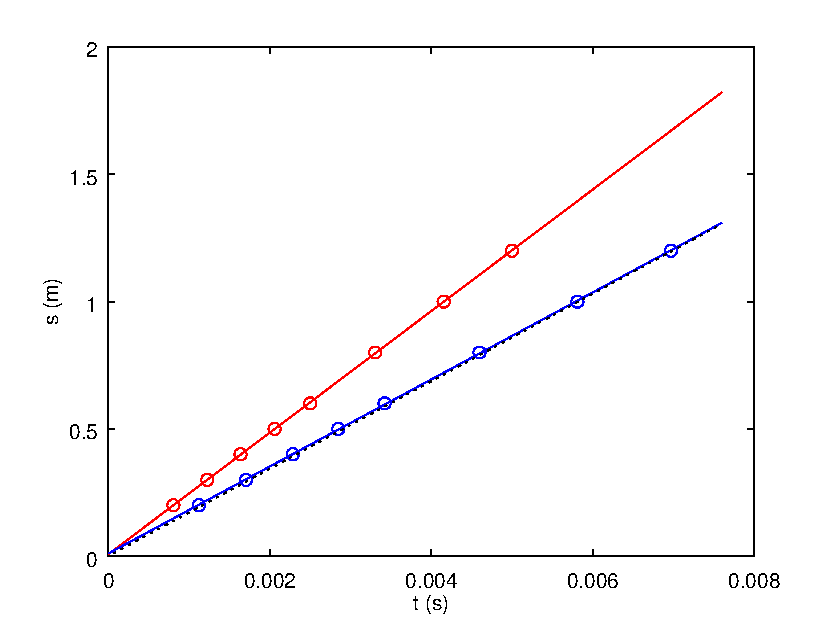
\includegraphics[scale=0.58]{sonar.pdf}
	\captionof{figure}{Valores experimentales erróneos (rojo) y correctos 
(azul). La recta punteada es el valor teórico.\label{fig:sonar_plot}}
\end{center}

Después de repasar el programa que muestra el tiempo que tarda el pulso de 
ultrasonidos en regresar, se ha detectado un error, provocado en una función de 
las bibliotecas de Arduino.

Resulta que la función \texttt{pulseIn} calcula el tiempo que dura un pulso, 
empleando un bucle, en el que se incrementa un contador. Luego multiplica las 
vueltas del bucle por el número de instrucciones que de antemano se han 
calculado. Sin embargo, el compilador \texttt{avr-gcc} puede alterar el número 
de instrucciones cuando se aplican optimizaciones. Este problema, provoca que el 
tiempo se vea alterado de la forma $ t_{real} = t * K $. Siendo $ K = 
1.3898 $, hallado de forma experimental.

Tras programar una nueva biblioteca para emplear el sensor de ultrasonidos, de 
forma independiente a las optimizaciones del código (empleando interrupciones), 
se vuelven a realizar las medidas.

%Para calcular el tiempo se realizan 100000 mediciones y se halla la media.

\begin{center}
\begin{tabular}{ | c | c | c | }
\hline
$s_{r}$ & $s_{t}$ & $t$\\ \hline
m & m & \si{\micro\second} \\ \hline \hline
0.20 & 0.193 & 1122 \\ \hline
0.30 & 0.293 & 1705 \\ \hline
0.40 & 0.392 & 2285 \\ \hline
0.50 & 0.489 & 2848 \\ \hline
0.60 & 0.588 & 3422 \\ \hline
0.80 & 0.789 & 4597 \\ \hline
1.00 & 0.998 & 5810 \\ \hline
1.20 & 1.197 & 6970 \\ \hline
\end{tabular}
\end{center}

Obteniendo por regresión lineal, de la misma forma, los coeficientes:
\begin{center}
\texttt{1.7084e+02   1.0857e-02}
\end{center}
Y por tanto, la recta característica es:
$$ s = 170.84 t + 1.0857\cdot 10^{-2} = 341.68\frac{t}{2} + 1.0857\cdot 10^{-2}
$$

Existe un error fijo de aproximadamente un centímetro (1.0857cm), que puede 
deberse a la dificultad de centrar la regla en el centro del sensor de 
ultrasonidos. Sin embargo, para determinar la distancia de un objeto al robot, 
esta distancia es despreciable.

Si comparamos la ecuación~\ref{eq:velocidad-sonido}, con el resultado 
experimental, despreciando el desplazamiento de 1cm, se puede observar que son 
muy similares.

La velocidad del sonido calculada de forma experimental, resulta ser 341,68 m/s.  
Este valor puede oscilar, ya que depende de la temperatura. Para calcular la 
temperatura:
$$ T = \frac{v_{s}-331.3}{0.606} = 17.129 \si{\celsius} $$
La temperatura registrada de la sala es de 18º. Por lo que se puede afirmar que 
el experimento muestra unos resultados esperados.

El error medio de distancia cometido, en el peor caso (a 1.20m de distancia 
real) es de unos 4mm.

Es importante mencionar, que un ajuste del error, empleando un método de 
regresión, permite solventar errores como el que ha sido detectado, pero no los 
corrige. Por ello, se ha decidido que si los cálculos teóricos, no concuerdan 
con los esperados, averiguar que ha causado el error.
\subsection{LDR}

El sensor LDR permite obtener una medida de la cantidad de luz que incide sobre 
el mismo. El robot dispone de dos sensores LDR. Uno ambiental, que está colocado 
en la parte superior, orientado hacia arriba. Además está cubierto por un 
cilindro cerrado de 4cm de altura, de plástico blanco translúcido. Esto le 
permite obtener una medida de la luz ambiente sin importar la dirección de donde 
proviene.

El sensor LDR direccional, se encuentra en la parte delantera orientado al 
frente. Este sin embargo, está encapsulado en un cilindro abierto, de plástico 
negro opaco. Lo cual le permite observar de forma direccional la luz que recibe 
por el frente, con el objetivo de encontrar una luz.
\subsubsection{\texttt{ldr0}: LDR ambiental}

Para calibrar el sensor ambiental, se realizarán algunas medidas comparando la 
distancia a un foco de luz. También se compararán los valores con distintos 
ángulos, para observar si realmente es invariante a la orientación.

El valor medido por el sensor, está representado en un intervalo $[0, 1024)$ de 
valores discretos. El valor 0, corresponde con un voltaje de 0V en la entrada de 
Arduino, y 1023 con +5V. De forma que si $l_0$ es el valor discreto medido por 
Arduino:
$$ V_0 = 5 \cdot \frac{l_0}{1023} $$
En la figura~\ref{fig:ldr_circuito} se observa el montaje del LDR $R_2$, junto 
con otra resistencia $R_1$ de un valor fijo de $10\si{\kohm}$.

\begin{center}
\begin{tikzpicture}
	\draw
		(0,0) to ++(0,-1) node[ground] {}
		(0,0) to[R, l_=$R_1$, -*] ++(2,0)
		to[short, -o] ++(0,-1) node[below] {$V_0$}

		(2,0) to[phR, l_=$R_2$] ++(2,0)
		to[short, -o] ++(0, -1) node[below] {V}
	;
\end{tikzpicture}
\captionof{figure}{Circuito del sensor LDR.\label{fig:ldr_circuito}}
\end{center}

%Para calcular el voltaje en $V_0$:
%$$ I = \frac{V}{R_T} = \frac{V}{R_1 + R_2} $$
%$$ V_{0} = I \cdot R_1 = V \frac{R_1}{R_1+R_2} = \frac{V}{1+\frac{R_2}{R_1}}$$
%Y posteriormente el valor de $R_2$:
%$$ R_{2} = R_1 \frac{V-V_0}{V_0}$$
%La relación entre la iluminación $I_V$ y la resistencia $R$ viene dada 
%por\footnote{\url{http://www.brighton-webs.co.uk/electronics/light\_dependent\_resistor.aspx}}:
%$$ \frac{E_2}{E_1} = \left(\frac{R_2}{R_1}\right)^\gamma$$
%Y entre la distancia $D$ y la iluminación:
%$$ \frac{E_1}{E_2} = \left(\frac{D_2}{D_1}\right)^2$$
%De forma que, para calcular el parámetro $\gamma$:
%$$ E_2 = E_1 \cdot \left( \frac{R_2}{R_1} \right) ^\gamma \Rightarrow 
%\left(\frac{R_2}{R_1} \right)^{-\gamma} = \left(\frac{D_2}{D_1}\right)^2$$
%$$ \gamma = \frac{2 \ln \frac{D_2}{D_1} }{-\ln\frac{R_2}{R_1}} $$
%
% TODO: Comprobar estas ecuaciones por algún libro.


Para calibrar el sensor ambiental, se realizarán algunas medidas observando el 
valor de la resistencia del LDR, mientras se varía la distancia del foco de luz, 
así como el ángulo.

En cada medida, el sensor realiza 5000 mediciones de forma contínua, y luego 
envía el valor de la media aritmética al ordenador, que es registrado.

En la tabla, $s$ indica la distancia a la fuente de luz. Los ángulos indican la 
orientación del robot:

\begin{center}
\begin{tabular}{ | c | c | c | c | c | }
\hline
$s$(m) & $0º$ & $-90º$ & $+90º$ & $+180º$ \\ \hline
0.20 & 936 & 926 & 933 & 943 \\ \hline
0.40 & 823 & 784 & 831 & 843 \\ \hline
0.60 & 719 & 675 & 729 & 742 \\ \hline
0.80 & 627 & 576 & 628 & 639 \\ \hline
1.00 & 555 & 505 & 560 & 531 \\ \hline
1.20 & 500 & 445 & 497 & 489 \\ \hline
1.40 & 429 & 396 & 446 & 454 \\ \hline
1.60 & 396 & 340 & 407 & 440 \\ \hline
1.80 & 378 & 296 & 383 & 405 \\ \hline
\end{tabular}
\end{center}

En la siguiente figura, se puede observar en una escala logarítmica para el eje 
y, el valor del sensor para cada orientación.

\begin{tikzpicture}
\begin{semilogyaxis}[grid=both,
	width=\columnwidth,
	height=0.4\textheight,
	xlabel = {Distancia a la luz (m)} ,
	ylabel = {Valor del sensor},
	xmin = 0.2, xmax = 1.8,
	ymin = 250, ymax = 1024,
	legend entries={$0º$,$-90º$,$90º$,$180º$},
	legend columns=4,
	legend style={
		at={(0.5,1.1)},
		anchor=north}
]
	\addplot+[smooth] table[x=x, y=0] {ldr0.csv};
	\addplot+[smooth] table[x=x, y=-90] {ldr0.csv};
	\addplot+[smooth] table[x=x, y=90] {ldr0.csv};
	\addplot+[smooth] table[x=x, y=180] {ldr0.csv};
\end{semilogyaxis}
\end{tikzpicture}

Existe una variación bastante marcada en la orientación de $-90º$. Esta 
variación indica que el sensor recibe menos luz de la esperada. Dicha variación 
está relacionada con la superficie del robot. Dado que hay cables en la 
superficie, cuando se coloca a $-90º$, los cables se sitúan entre la luz y el 
sensor, y provocan una disminución de la intensidad.

En las demás orientaciones no se producen grandes cambios. Por lo que se asume 
que el sensor es realmente independiente de la orientación.
\subsubsection{\texttt{ldr1}: LDR direccional}
El sensor LDR direccional, por el contrario, trata de aumentar la variación de 
la luz conforme a la orientación. Para calibrar este sensor se realizará un 
experimento similar, dividido en 4 orientaciones. Se asume que los valores para 
los ángulos opuestos, dada la simetría, son iguales.

Se muestran en la siguiente tabla los resultados obtenidos:

\begin{center}
\begin{tabular}{ | c | c | c | c | c | }
\hline
$s$(m) & $0º$ & $30º$ & $60º$ & $90º$ \\ \hline
0.10 & 1015 & 1011 & 1004 & 977 \\ \hline
0.20 & 1015 & 998 & 670 & 404 \\ \hline
0.30 & 1013 & 915 & 520 & 414 \\ \hline
0.40 & 1011 & 838 & 416 & 314 \\ \hline
0.50 & 1008 & 684 & 308 & 254 \\ \hline
0.60 & 1004 & 534 & 216 & 202 \\ \hline
0.70 & 999 & 500 & 214 & 113 \\ \hline
0.80 & 996 & 394 & 188 & 95 \\ \hline
0.90 & 992 & 355 & 164 & 80 \\ \hline
1.00 & 987 & 352 & 136 & 70 \\ \hline
1.20 & 977 & 277 & 96 & 60 \\ \hline
1.40 & 968 & 173 & 65 & 57 \\ \hline
\end{tabular}
\end{center}

Finalmente, en la figura~\ref{fig:ldr1}, se muestran también en una escala 
logarítmica para el valor del sensor.

\begin{figure}[h]
\centering
\begin{tikzpicture}
\begin{semilogyaxis}[grid=both,
	width=\columnwidth,
	height=0.4\textheight,
	xlabel = {Distancia a la luz (m)} ,
	ylabel = {Valor del sensor},
	xmin = 0, xmax = 1.4,
	ymin = 0, ymax = 1100,
	legend entries={0º,30º,60º,90º},
	legend columns=4,
	legend style={
		at={(0.5,1.1)},
		anchor=north}
]
	\addplot+[smooth] table[x=x, y=0] {ldr1.csv};
	\addplot+[smooth] table[x=x, y=30] {ldr1.csv};
	\addplot+[smooth] table[x=x, y=60] {ldr1.csv};
	\addplot+[smooth] table[x=x, y=90] {ldr1.csv};
\end{semilogyaxis}
\end{tikzpicture}
\caption{Resultados del experimento de calibración de 
\texttt{ldr1}.\label{fig:ldr1}}
\end{figure}
\subsection{\texttt{mouse0}: Ratón de bola}

En la parte posterior, un ratón de bola permite obtener mediciones del movimiento del
robot. Tiene un controlador EM83702BP, que dispone con dos contadores digitales que
realizan la medición del desplazamiento en el eje $x$ e $y$.

Una bola de goma se encuentra en contacto con el suelo. Al desplazar el ratón, 
la bola gira alrededor de un eje imaginario, que es perpendicular al sentido del
desplazamiento y paralelo al suelo. Desplazándose en la dirección de $\vec{m}$.

Ya que los movimientos efectuados por el robot serán los que provoquen sus dos ruedas,
se puede determinar la posición, midiendo sólo el desplazamiento del ratón. Para ello,
se observa en la figura~\ref{fig:giro} un ejemplo de un giro de $\alpha = \RobotAngleº$.


\subsubsection{Movimiento de la bola}
Para poder analizar el movimiento que realizará el robot, mediante la 
información que el ratón proporciona, es necesario conocer como varía el vector 
$\vec{m}$ que indica el desplazamiento real del ratón, con respecto a la 
información proporcionada por el mismo.

Para ello, es necesario averiguar el funcionamiento del ratón. Este consta de 
una bola de goma, que está situada en un zócalo, donde puede girar libremente, 
al mover el ratón por una superficie.

Dos rodillos de plástico rozan con la bola, situados en un ángulo de $90º$. A 
continuación se analiza, como el movimiento de la bola, roza en los puntos $B_1$ 
y $B_2$ con los rodillos del ratón. En la figura~\ref{fig:bola} se observa con 
detalle el mismo giro que en la figura~\ref{fig:giro}.

% TODO: Poner los ejes en la figura y R

\begin{figure}[h]
\centering
\begin{tikzpicture}[>=latex, semithick]
	\pgfmathsetmacro{\BallRadius}{3.0}%
	\pgfmathsetmacro{\BallOptoL}{2}%
	\pgfmathsetmacro{\BallOptoD}{0.6}%
	\pgfmathsetmacro{\BallBeta}{atan(\RobotSize/\RobotRadius)}%
	\pgfmathsetmacro{\BallBetaDouble}{90.0-\BallBeta*2.0}%

	\draw circle(\BallRadius);
	\fill [black] (0,0) coordinate [label=below:$O$] (O) circle (1pt);
	%Puntos de choque
	\fill [black] (0,-\BallRadius) coordinate [label=below:$B_1$] (Bx) circle (1pt);
	\fill [black] (-\BallRadius,0) coordinate [label=left:$B_2$] (By) circle (1pt);
	%Ejes
	\draw[dotted] (-\BallRadius,0) -- (\BallRadius,0);
	\draw[dotted] (0,\BallRadius) -- (0,-\BallRadius);

	%Radio de la bola
	\draw[] (O) -- +(-\BallRadius,0) node[pos=0.5,auto=left]{$R_b$};
	%Cilindros de los ejes
	\draw[] (By) +(-\BallOptoD,-\BallOptoL) rectangle +(0,\BallOptoL);
	\draw[] (Bx) +(-\BallOptoL,-\BallOptoD) rectangle +(\BallOptoL,0);
	%Puntos
	\fill[black] (180-\BallBeta*2:\BallRadius) coordinate [label=above:$C_2$] (Cy) circle (1pt);
	\draw[blue] (By) -- (Cy) node[pos=0.5,auto=right]{$d_2$};
	\fill[black] (90-\BallBeta*2:\BallRadius) coordinate [label=right:$C_1$] (Cx) circle (1pt);
	\draw[blue] (Bx) -- (Cx) node[pos=0.5,auto=right]{$d_1$};
	%Ángulos
	%\draw[dotted] (Bx) +(-90:\BallRadius/5) arc
	%(-90:-90-\BallBeta:\BallRadius/5.0) node[pos=0,auto=left]{$\beta$};

	%\draw[dotted,rotate=90-\BallBeta]
	%	($0.5*(By)+0.5*(Cy)$) ellipse (1.35 and 0.15)
	%	($0.5*(Bx)+0.5*(Cx)$) ellipse (2 and 0.15);
	%\coordinate (C3) at ($0.5*(C1)+0.5*(C2)$)


	% Angulos del eje x
	\begin{scope}
		\path[clip] (Bx) -- (O) -- (Cx) -- cycle;
		\draw (Bx) circle (\BallRadius/3);
		\node[above] at ($(Bx) +(+90-\BallBeta/2:\BallRadius/3)$) {$\beta$};
		\draw (O) circle (\BallRadius/5);
		\node[right] at ($(O) +(-\BallBeta:\BallRadius/5)$) {$\gamma$};
	\end{scope}

	%Ángulos del eje y
	\begin{scope}
		\path[clip] (By) -- (O) -- (Cy) -- cycle;
		\draw (By) circle (\BallRadius/5);
		\node[right] at ($(By) +(+45-\BallBeta/2:\BallRadius/5)$) {$\delta$};
		\draw (O) circle (\BallRadius/5);
		\node[left] at ($(O) +(+180-\BallBeta:\BallRadius/5)$) {$\theta$};
	\end{scope}

	%Dibujar el vector del raton
	\draw[red,-latex,shorten >=1pt] (O) -- +(90-\BallBeta:\BallRadius/2)
		node[pos=0.5,auto=left]{$\vec{m}$};

	\draw[dotted] (O) -- (Cx);
	%\draw[dotted] (Cx) +(270.0-\BallBeta:\BallRadius/5) arc (90.0-\BallBeta:\BallBetaDouble:\BallRadius/5.0) node[auto=right]{$\beta$};

	%\draw[dotted] (O) +(\BallBetaDouble:\BallRadius/4.0) arc (\BallBetaDouble:-90.0:\BallRadius/4.0) node[auto=right,pos=0.5]{$\delta$};

	\draw[dotted] (O) -- (Cy);
	%\draw[dotted] (O) +(90.0+\BallBetaDouble:\BallRadius/6.0) arc (90.0+\BallBetaDouble:180.0:\BallRadius/6.0) node[auto=above]{$\theta$};
	%node[auto=left,pos=0.5]{$\theta$}



\end{tikzpicture}
\captionof{figure}{Diagrama de la bola del ratón.\label{fig:bola}}
\end{figure}
\subsubsection{El tamaño de la bola}

¿Cómo se mueven los rodillos del ratón, cuando la bola gira? Para responder a 
esta cuestión, se moverá el ratón un desplazamiento $\vec{m}$ a una velocidad 
uniforme y en línea recta, y se intentará calcular de forma teórica el resultado 
esperado.

Los ejes están intercambiados con respecto al orden habitual de un plano. Esto 
es debido a que el ratón está colocado en el robot como en la 
figura~\ref{fig:bola}. Sin embargo mantienen el sentido. Hacia arriba y derecha 
son positivos.

El rodillo inferior, girará rozando continuamente por el punto $B_1$ a medida 
que la bola gire. Dado que la dirección $\vec{m}$ permanece constante durante 
este movimiento, el punto $B_1$ describirá una trayectoria circular en la 
superficie de la bola. La bola tiene un radio $R_b$.

El perímetro de esta circunferencia se denomina por $p_1$, que es tangente a 
$B_1$ y $C_1$ y que tiene por diámetro $d_1$. De modo que cuando la bola dé una 
vuelta completa, el rodillo habrá avanzado exactamente $p_1$.

La distancia $d_1$ es la cuerda de ángulo $\gamma$, cuya longitud es, por su 
propia definición:
$$ d_1 = R_b \, \text{crd} \, \gamma = 2R_b \sin \frac{\gamma}{2}$$
Además, el ángulo $\gamma = 180º - 2\beta$, pues forma un triángulo isósceles:
$$ d_1 = 2R_b \sin(90-\beta) = 2R_b\cos \beta$$
De igual modo para $d_2$:
$$ d_2 = R_b \, \text{crd} \, \theta = 2R_b \sin \frac{\theta}{2} $$
Sabiendo que $\theta = 180º - 2\delta$ y que $\beta = 90 - \delta$, puesto que 
$d_1 \parallel d_2$:
$$ d_2 = 2R_b \sin (90 - \delta) = 2R_b \sin \beta $$
Finalmente, para los perímetros:
$$ p_1 = \frac{2\pi d_1}{2} = 2 \pi R_b\cos \beta \quad  p_2 = \frac{2\pi 
d_2}{2} = 2 \pi R_b\sin \beta $$

Si se supone que no hay ningún deslizamiento entre la bola y el rodillo, cuando 
la bola avance $\vec{m}$, ésta girará un ángulo $\theta_b$:
$$ \theta_b = \frac{m}{R_b} $$

Si $R_r$ es el radio de los rodillos, estos girarán un ángulo:
$$ \theta_1 = \frac{\theta_b d_1}{2R_r} \quad
	\theta_2 = \frac{\theta_b d_2}{2R_r}$$
Sustituyendo $d_1$ y $d_2$:
$$ \theta_1 = \frac{\theta_b 2R_b\cos \beta}{2R_r} =
	\frac{R_b}{R_r}\theta_b\cos \beta$$
$$ \theta_2 = \frac{\theta_b 2R_b\sin \beta}{2R_r} =
	\frac{R_b}{R_r}\theta_b\sin \beta$$
Recuperando el valor de $\theta_b$, el radio $R_b$ desaparece:
\begin{equation}
\theta_1 = \frac{m \cos \beta}{R_r} \quad
\theta_2 = \frac{m \sin \beta}{R_r} \label{eq:bola-angulo}
\end{equation}
De modo que se obtiene una relación entre el ángulo con el que se desplaza el 
ratón y el giro de cada uno de los rodillos, como se deseaba. Además se observa 
que el tamaño no importa, de la bola, para calcular el giro de los rodillos.
\subsubsection{Los optoreceptores}

Los rodillos que rozan con la bola, tienen en los extremos unos discos con
ranuras equiespaciadas, de modo que cortan un haz de luz infrarrojo al girar.  
Este efecto, provoca que un sensor registre el número de veces que se ha cortado 
el haz, y por lo tanto mide, de forma discreta, cuánto ha girado el rodillo, es 
decir $\theta_1$ y $\theta_2$.

%TODO:Incluir diagrama de los dientes y las gráficas

Cada disco tiene 27 dientes y $R_r$, el radio de los rodillos, es de 
1.4$\pm$0.1 mm.

Además, en cada disco se encuentran dos receptores, desfasados 90º, de forma que 
pueden detectar el sentido de giro. Por cada diente que se avanza, se cuentan 4 
pasos en los contadores digitales.

Si $o_1$ y $o_2$ son los valores medidos por los contadores que acumulan el 
número de pasos que se ha desplazado el rodillo:
$$o_1 = \frac{27 \cdot 4 \theta_1}{2\pi} \quad 
o_2 = \frac{27 \cdot 4 \theta_2}{2\pi}$$

Sustituyendo el valor del ángulo $\theta_1$ y $\theta_2$ por la 
ecuación~\ref{eq:bola-angulo}:
$$ o_1 = \frac{27\cdot4}{2 \pi R_r} m \cos \beta \quad
	o_2 = \frac{27\cdot4}{2 \pi R_r} m \sin \beta $$

Añadiendo una constante $K_r$:
$$K_r = \frac{27\cdot4}{2 \pi R_r} = 12\pm2$$
$$ o_1 = K_r m \cos \beta \quad
	o_2 = K_r m \sin \beta $$
Esta constante, $K_r$, ha sido calculada de forma experimental, con un valor de 
11,484. Este valor se encuentra dentro del margen calculado, por lo que se 
considera como válido, y verifica los cálculos realizados.
$$K_r = 11,484$$
Para calcular esta constante, se realizó un movimiento de 150mm, en línea recta 
y se registraron los valores de $o_1$, que mide el desplazamiento en el eje $y$:

\begin{center}
\begin{tabular}{ | c | c | c | c | c | c |}
\hline
$o_1$ & 1719 & 1728 & 1722 & 1719 & 1725 \\ \hline
\end{tabular}
\end{center}

Tras calcular la media, y dividirla por 150mm, se obtiene el valor $K_r$.

Empleando una notación vectorial, $\vec{o}$ es el desplazamiento indicado por el 
ratón, tras intercambiar sus ejes: $\vec{o} = (o_2, o_1)$.

De forma que $o_x = o_2 = K_r m \sin \beta$ y $o_y = o_1 = K_r m \cos \beta$. Ya 
que $m_x = m \sin \beta$ y $m_y = m \cos \beta$, se simplifica: $o_x = K_r m_x$ 
y $o_y = K_r m_y$, quedando finalmente:
\begin{equation}
	\vec{o} = K_r \vec{m} \Longrightarrow \vec{m} = \frac{\vec{o}}{K_r}
	\label{eq:o}
\end{equation}
\subsubsection{El radio de giro $R_r$}

\begin{figure}[h]
\centering
\begin{tikzpicture}[>=latex,semithick]
	%\path[draw] (-4,0)  coordinate [label= left:$A$] (A)
	%        -- ( 0,4)  coordinate [label=above:$C$] (C)
%        -- ( 4,0)  coordinate [label=right:$B$] (B)
	%        -- cycle;
	%\foreach \point in {A,B,C}
	%       \fill [black] (\point) circle (2pt);
	%\draw [color=red] circle(4cm);


	%\draw (A) rectangle (1,1);

	%\def\robotsize{(1,1)}
	%\pgfmathsetmacro{\RobotSize}{2.0}%
	%\pgfmathsetmacro{\RobotAngle}{-45.0}%
	%\pgfmathsetmacro{\RobotRadius}{6.0}%
	\pgfmathsetmacro{\RobotBall}{0.15}%
	\pgfmathsetmacro{\RobotOC}{sqrt(\RobotSize*\RobotSize +
		\RobotRadius*\RobotRadius)}%
	\pgfmathsetmacro{\RobotAngleAOC}{atan(\RobotSize/\RobotRadius)}%
	\def\BallBeta{\RobotAngleAOC}


	\fill [black] (0,0) coordinate [label=left:$O$] (O) circle (1pt);
	\fill [black] (0:\RobotRadius) coordinate [label=below:$A_1$] (A1)
		circle (1pt);
	\fill [black] (\RobotAngle:\RobotRadius) coordinate [label=above:$A_2$] (A2)
		circle (1pt);
	\fill (A1) +(0,-\RobotSize) coordinate [label=below:$C_1$] (C1) circle (1pt);
	\fill[rotate=\RobotAngle] (A2) +(0,-\RobotSize) coordinate [label=above:$C_2$]
		(C2) circle (1pt);


	\draw[dotted] (O) -- (A1);
	\draw[dotted] (O) -- (A2);
	\draw[dotted] (O) -- (C1);

	% Ángulos
	\draw[blue] (\RobotRadius/5,0) arc (0:\RobotAngle:\RobotRadius/5.0)
		node[pos=0.5,auto=right]{$\alpha$};
	\draw[red] (\RobotRadius/5,0) arc (0:-\RobotAngleAOC:\RobotRadius/5.0)
		node[pos=0.5,auto=left]{$\beta$};
	\draw[magenta] (A1) +(-\RobotRadius/5,0)
		arc (180:90+\RobotAngle/2:\RobotRadius/5.0)
		node[pos=0.5,auto=left]{$\gamma$};
	\draw[violet] (A1) +(\RobotRadius/8,0)
		arc (0:(180+\RobotAngle)/2:\RobotRadius/8.0)
		node[pos=0.5,auto=left]{$\phi$};

	% Dibujar el robot en A1
	\draw[] (A1) +(-\RobotSize/2,0) rectangle +(\RobotSize/2,-\RobotSize);
	\draw[dotted] (C1) circle(\RobotBall);

	%Dibujar el robot en A2
	\draw[rotate=\RobotAngle] (A2) +(-\RobotSize/2,0)
		rectangle +(\RobotSize/2,-\RobotSize);
	\draw[dotted] (C2) circle(\RobotBall);

	%Trayectoria raton
	%\pgfmathsetmacro{\XValueArc}{\ArcRadius*cos(\ArcAngle)}%
	\draw[blue] (C1) arc (-\RobotAngleAOC:\RobotAngle-\RobotAngleAOC:\RobotOC)
		node[pos=0.7,auto=right]{$a$};

	%\draw (0,0) coordinate [label=right:$O$] (O) circle(4);
	\draw[dotted] (A1) arc (0:\RobotAngle:\RobotRadius);
	\draw[-latex,shorten >=1pt] (A1) -- (A2) node[pos=0.5,auto=right]{$\vec{r}$};

	%Dibujar el vector del raton
	\draw[red,-latex,shorten >=1pt] (C1) -- +(90-\RobotAngleAOC:\RobotRadius/3)
		node[pos=0.5,auto=right]{$\vec{m}$};


\end{tikzpicture}
\captionof{figure}{Diagrama de un giro del robot.\label{fig:giro}}
\end{figure}
Para calcular el radio de giro $R_r$ del robot se empleará el triángulo 
$OA_1C_1$ que comparte el lado $R_r$ con el triángulo $OA_2A_1$.

$l$ es la distancia que separa el ratón del eje de las ruedas, $l = 
\overline{A_1C_1}$. $R_m$ es el radio desde el $O$ hasta el ratón, $C_1$.

Observando el ángulo $\beta$ se cumple que:
\begin{equation}
	\sin \beta = \frac{l}{R_m} = \frac{m_x}{m} \Longrightarrow
		R_m = \frac{l \cdot m}{m_x}
\label{eq:Rm}
\end{equation}

Ahora, tomando el triángulo $OA_1C_1$:
\begin{equation}
	R_r = R_m cos \beta = R_m \frac{m_y}{m} =
		\frac{l \cdot m \cdot m_y}{m_x \cdot m} =
		\frac{l \cdot m_y}{m_x}
\label{eq:Rr}
\end{equation}
\subsubsection{El ángulo $\alpha$}
En un giro el robot mueve el ratón en la trayectoria descrita por el arco $a$, 
como muestra la figura~\ref{fig:giro}. Dado que el ratón gira acompañando al 
robot, la trayectoria percibida por el mismo, es en línea recta, y de una 
longitud exactamente igual a $a$. De forma que:
$$m = \sqrt{m_x^2 + m_y^2} = a$$
Si $R_m = \overline{OC_1}$, dado que  $\alpha = \widehat{A_1OA_2} = 
\widehat{C_1OC_2}$, se tiene que $a = \alpha R_m$. Junto con lo anterior:
$$ m = \alpha R_m $$
Empleando la ecuación~\ref{eq:Rm}:
\begin{equation}
	\alpha = \frac{m}{R_m} = \frac{m \cdot m_x}{l \cdot m} = \frac{m_x}{l}
	\label{eq:alpha}
\end{equation}
\subsubsection{El vector $\vec{r}$}
Para determinar la posición del robot, es necesario calcular el vector 
$\vec{r}$. Este vector indica el deplazamiento del robot, usando un sistema de 
coordenadas local. Observando el ángulo $\phi$:
$$r_x = r \cos \phi \quad
r_y = r \sin \phi $$
En forma matricial, empleando $R_\phi$ como matriz de rotación:
\begin{equation}
\vec{r} =
\begin{bmatrix}
r_x\\
r_y
\end{bmatrix}
=
R_\phi
\begin{bmatrix}
r\\
0
\end{bmatrix}
=
\begin{bmatrix}
\cos \phi & -\sin \phi \\
\sin \phi & \cos \phi \\
\end{bmatrix}
\begin{bmatrix}
r\\
0
\end{bmatrix}
\label{eq:r_matrix}
\end{equation}
Y ya que $r$ es la cuerda de radio $R_r$ y ángulo $\alpha$, se tiene que:
$$ r = R_r \, \text{crd} \, \alpha = 2 R_r \sin \frac{\alpha}{2} $$
Junto con las ecuaciones \ref{eq:alpha} y \ref{eq:Rr}:
$$ r = 2 R_r \sin \frac{m_x}{2l} =
	\frac{2 l m_y}{m_x} \sin \frac{m_x}{2l}$$
Dado que existe una división por $m_x$ que valdrá 0 cuando el robot avance en 
el eje $y$, es necesario evitar la división por cero:

\begin{equation}
r = \begin{dcases}
		\frac{2 l m_y}{m_x} \sin \frac{m_x}{2l} & \text{si } m_x \ne 0 \\[1mm]
		m_y & \text{si } m_x = 0 \\
	\end{dcases}
\label{eq:r}
\end{equation}
\subsubsection{El ángulo global $\theta$}
En cada giro, el ángulo global $\theta$ cambia, y ha de actualizarse. Se 
denomina $\Delta \theta$ al giro que se produce en un intervalo $\Delta t$, tras 
cada actualización.
$$ \theta(t + \Delta t) = \theta(t) + \Delta \theta $$
Observando la figura~\ref{fig:giro}, ángulo $\alpha$ indica el giro que describe 
el robot, en $\Delta t$, por lo que $\Delta \theta = \alpha$:
\begin{equation}
	\theta(t + \Delta t) = \theta(t) + \alpha
\end{equation}
Siendo $\alpha$ el ángulo que gira el robot entre $t$ y $t + \Delta t$.

\subsubsection{La posición global $\vec{s}$}
El vector $\vec{s}(t)$ indica la posición global del robot en el instante $t$, 
tomando un sistema de coordenadas globales:
$$
	\vec{s}(t + \Delta t) =
		\vec{s}(t) + \Delta \vec{s}
$$

En cada movimiento del robot avanzará $\vec{r}$ en el sistema de coordenadas del 
robot. De forma que para calcular $\Delta\vec{s}$:
$$
	\Delta\vec{s} = R_{\theta(t)} \cdot \vec{r}
$$
El ángulo $\theta$ indica el giro global del robot, $\theta = \alpha $.

Substituyendo $\vec{r}$ por la ecuación~\ref{eq:r_matrix}:
$$
	\Delta\vec{s} = R_{\alpha} \cdot R_{\phi} \cdot
			\begin{bmatrix}
				r \\
				0
			\end{bmatrix}
		= R_{\alpha + \phi} \cdot
			\begin{bmatrix}
				r \\
				0
			\end{bmatrix}
$$
Realizando la multiplicación de la matriz:
$$
	\Delta s_x = r\cos(\alpha + \theta) \quad
	\Delta s_y = r\sin(\alpha + \theta)
$$

De forma que en cada $\Delta t$, la posición de actualizará:
\begin{equation}
\begin{split}
	s_x(t + \Delta t) = s_x(t) + r\cos(\alpha + \theta) \\
	s_y(t + \Delta t) = s_y(t) + r\sin(\alpha + \theta)
\end{split}
\end{equation}

\subsubsection{Odometría}
Para determinar la ubicación del robot, bastará con conocer la posición y el 
ángulo del robot. De forma que $\theta_r$ indicará el ángulo del robot de forma 
global, y $\vec{s}$ su posición.

En cada giro, el robot cambiará su orientación en $\Delta\theta_r = \alpha$. De 
forma que empleando la ecuación~\ref{eq:alpha}:
$$ \theta_r = \sum \Delta \theta_r = \sum \alpha = \sum \frac{m_y}{l}$$

Para el vector $\vec{s}$, para cada giro:
$$ \vec{s} = \sum \Delta \vec{s} = \sum \vec{r} $$









\section{Posibles errores}

La función \texttt{attachInterrupt} no borra las banderas (flags) \texttt{INTF0} 
y \texttt{INTF1} del registro \texttt{EIFR}, de forma que al colocar una 
interrupción por primera vez, es posible que se ejecute al comienzo sin haber 
recibido tal interrupción. Una posible solución es añadir esta línea al comienzo 
de la función:

\texttt{EIFR |= \_BV(INTF0) || \_BV(INTF1);}

La función \texttt{pulseIn} calcula el tiempo dependiendo de las optimizaciones
que se produzcan. Es necesario que sea independiente. Además es conveniente
sustituirla por alguna función no bloqueante que emplee interrupciones.
\section{TODO}
Este documento está incompleto. Faltan cálculos en la parte de la odometría, así 
como los experimentos que verifican la posición de robot.

Falta cambiar los gráficos a pgf. Corregir la ortografía. Usar la precisión en 
los experimentos. Encontrar la ecuación que describe la luz con la distancia, en 
el LDR. Y las ecuaciones que describen el movimiento de los motores, sabiendo el 
voltaje y tiempo de funcionamiento.

La última versión se encuentra en \url{https://github.com/rodarima/robotica}.
\end{document}
